\chapter{Sistemas de excitación. Control tensión-reactiva.}
	\section{Respuesta de sistemas.}
		\subsection{Sistemas de primer orden.}
			Sea el sistema con realimentación unitaria de la figura siguiente:
			\begin{figure}[H]
				\centering
					\begin{circuitikz}[scale=0.7]
						\tikzstyle{every node}=[font=\normalsize]
						\draw  (9.75,14) circle (0.5cm);
						\draw [->, >=Stealth] (7.75,14) -- (9.25,14)node[pos=0.25,above]{X(s)};
						\draw [->, >=Stealth] (10.25,14) -- (11.25,14);
						\draw  (11.25,14.75) rectangle  node {\normalsize G(s)} (13.5,13.25);
						\draw [short] (14.5,14) -- (14.5,12.5);
						\draw [short] (14.5,12.5) -- (9.75,12.5);
						\draw [->, >=Stealth] (9.75,12.5) -- (9.75,13.5);
						\node [font=\normalsize] at (9,14.25) {+};
						\node [font=\normalsize] at (10,13.25) {-};
						\node at (14.5,14) [circ] {};
						\draw [->, >=Stealth] (13.5,14) -- (15.5,14)node[pos=0.5,above]{Y(s)};
					\end{circuitikz}
			\end{figure}
			
			$G(s)$ se denomina "función de transferencia de la planta", y su comportamiento viene descrito por los polos y ceros que lo componen:
			\[G(s) = \dfrac{\prod ceros}{\prod polos} = \dfrac{b_0 + b_1 s + b_2 s^2\dots + b_m s^m}{a_0 + a_1 s + a_2 s^2\dots + a_n s^n}\]
			El sistema será estable si, en la función de transferencia global, el número de polos es mayor al de ceros: $n>m$.
			
			La función de transferencia del sistema es:
			\[M(s) = \dfrac{Y(s)}{X(s)} = \dfrac{G(s)}{1 + G(s)}\]
			
			
			Si una función $G(s)$ es de primer orden es de la forma:
			\[G(s) = \dfrac{K}{1+Ts} = \dfrac{\dfrac{K}{T}}{s+\dfrac{1}{T}}\]
			Donde $K$ es la ganancia del sistema (su valor cuando finaliza el transitorio) y $T$ la constante de tiempo del sistema.
			
			
			La respuesta a escalón de un sistema de primer orden es:
			\[y(t) = K\left(1-e^{-t/T}\right)\]
			
			
			Los sistemas de primer orden tienen un polo. Si el polo es positivo entonces el sistema es inestable, si es negativo es estable y si es 0 el sistema no converge y es críticamente estable:
			\begin{figure}[H]
				\begin{minipage}{0.5\textwidth}
					\begin{figure}[H]
						\centering
						\begin{circuitikz}
							\tikzstyle{every node}=[font=\normalsize]
							\draw [->, >=Stealth] (11.25,13) -- (15.5,13)node[pos=1,above]{Re};
							\draw [->, >=Stealth] (13.25,12.5) -- (13.25,15)node[pos=1,above]{Im};
							\node at (12.25,13) {$\times$};
							\draw [ color={rgb,255:red,0; green,128; blue,0}, ->, >=Stealth, dashed] (13,14.5) -- (11.25,14.5)node[pos=0.5,above]{Estable};
							\draw [ color={rgb,255:red,255; green,0; blue,0}, ->, >=Stealth, dashed] (13.5,14.5) -- (15.5,14.5)node[pos=0.5,above]{Inestable};
						\end{circuitikz}
						
						\label{fig:my_label}
					\end{figure}
				\end{minipage}
				\begin{minipage}{0.5\textwidth}
					\begin{figure}[H]
						\centering
						\begin{circuitikz}[scale = 0.8]
							\tikzstyle{every node}=[font=\normalsize]
							\draw [->, >=Stealth] (13.75,12.75) -- (17.5,12.75)node[pos=1,above]{t};
							\draw [->, >=Stealth] (14,12.5) -- (14,16)node[pos=1,right]{y};
							\draw [ color={rgb,255:red,0; green,128; blue,255}, short] (14,12.75) .. controls (14.25,14) and (14.25,15.5) .. (17.25,15.5);
							\draw [dashed] (17.25,15.5) -- (14,15.5)node[pos=1,left]{K};
						\end{circuitikz}
						
						\label{fig:my_label}
					\end{figure}
				\end{minipage}
			\end{figure}
			
			
			
			
		\subsection{Sistemas de segundo orden subamortiguados.}
			Sea el sistema con realimentación unitaria de la figura anterior. Si ahora $G(s)$ tiene 2 polos será de segundo orden. La posición de los polos de la función de transferencia del lazo abierto determina el lugar de las raíces, que muestra el comportamiento del sistema: si son complejos conjugados será subamortiguado.
			
			\begin{figure}[H]
				\begin{minipage}{0.5\textwidth}
					\[G(s) = \dfrac{K \omega_n^2}{s^2 + 2\xi \omega_n s + \omega_n^2}\]
					\[\sigma = \xi \omega_n \qquad \xi = \cos \theta\]
				\end{minipage}
				\begin{minipage}{0.5\textwidth}
					\begin{figure}[H]
						\centering
						\begin{circuitikz}
							\tikzstyle{every node}=[font=\normalsize]
							\draw [->, >=Stealth] (11.25,13) -- (14,13)node[pos=1,above]{Re};
							\draw [->, >=Stealth] (13.25,11) -- (13.25,15)node[pos=1,above]{Im};
							\node at (11.75,14.25) {$\times$};
							\node at (11.75,11.75) {$\times$};
							\draw [short] (13.25,13) -- (11.75,14.25)node[pos=0.5,above, sloped]{$\omega_n$};
							\draw [dashed] (11.75,14.25) -- (13.25,14.25)node[pos=1,right]{$j\omega_d$};
							\draw [dashed] (11.75,14.25) -- (11.75,11.75)node[pos=0.4,left]{$\sigma$};
							\draw [short] (11.75,11.75) -- (13.25,13);
							\draw [<->, >=Stealth] (12.5,13.6) .. controls (12.25,13.3) and (12.25,13.25) .. (12.25,13)node[pos=0.5,left]{$\theta$};
							\draw [ color={rgb,255:red,0; green,128; blue,255}, short] (11.75,11.75) -- (11.75,11);
							\draw [ color={rgb,255:red,0; green,128; blue,255}, short] (11.75,14.25) -- (11.75,15);
						\end{circuitikz}
						
						\label{fig:my_label}
					\end{figure}
				\end{minipage}
			\end{figure}
			
			Respuesta a escalón en sistemas subamortiguados ($0 <\xi < 0.707$):
			\[y(t) = K\left(1-\dfrac{e^{-\sigma t}}{\sqrt{1-\xi^2}} \sin (\omega_d t + \theta)\right)\]
			
			\begin{figure}[H]
				\begin{minipage}{0.5\textwidth}
					\begin{itemize}
						\item \textbf{\textit{Tiempo de establecimiento:}} tiempo que tarda en llegar al valor final con un error del 5\%: \[t_s = \dfrac{\pi}{\sigma}\]
						\item \textbf{\textit{Tiempo de pico:}} \[t_p = \dfrac{\pi}{\omega_d}\]
						\item \textbf{\textit{Sobreoscilación:}} \[M_p = e^{-\pi/\tan \theta}\cdot 100\%\]
						\item \textbf{\textit{Tiempo de subida:}} tiempo que tarda en alcanzar el 100\% desde el inicio del transitorio: \[t_r = \dfrac{\pi - \theta}{\omega_d}\]
					\end{itemize}
				\end{minipage}
				\begin{minipage}{0.5\textwidth}
					\begin{figure}[H]
						\centering
							\begin{circuitikz}[scale = 1.3]
								\tikzstyle{every node}=[font=\normalsize]
								\draw [->, >=Stealth] (13.75,12.75) -- (17.5,12.75)node[pos=1,above]{t};
								\draw [->, >=Stealth] (14,12.5) -- (14,16)node[pos=1,right]{y};
								\draw [ color={rgb,255:red,0; green,128; blue,255}, short] (14,12.75) .. controls (14.25,15) and (14.5,16) .. (15,14.75);
								\draw [dashed] (17.25,14.75) -- (14,14.75)node[pos=1,left]{K};
								\draw [ color={rgb,255:red,0; green,128; blue,255}, short] (15,14.75) .. controls (15.5,13.5) and (15.5,15.75) .. (16,14.75);
								\draw [ color={rgb,255:red,0; green,128; blue,255}, short] (16,14.75) .. controls (16.5,14) and (16.5,15.25) .. (16.75,14.75);
								\draw [dashed] (14.6,15.3) -- (14.6,12.75)node[pos=1,below]{$t_p$};
								\draw [dashed] (15.75,15) -- (15.75,12.75)node[pos=1,below]{$t_s$};
								\draw [dashed] (14.3,14.75) -- (14.3,12.75)node[pos=1,below]{$t_r$};
								\draw [dashed] (14.6,15.3) -- (14,15.3)node[pos=1,left]{$K \cdot M_p$};
							\end{circuitikz}
						
						\label{fig:my_label}
					\end{figure}
				\end{minipage}
			\end{figure}
			
			
		\subsection{Sistemas de tercer orden.}
			Constan de tres polos. Se distinguen, por simplificar, 2 casos fundamentales:
			\begin{itemize}
				\item \textbf{\textit{Tres polos reales:}}
				 	La salida de la función de transferencia tendrá 3 componentes de la forma:
				 	\[A_1 e^{s_1 t},\,A_2 e^{s_2 t},\,A_3 e^{s_3 t}\]
				 	
				 	Luego para que el sistema sea estable $s_1$, $s_2$ y $s_3$ deben ser negativos en su parte real.
				 	
				 \item \textbf{\textit{Un polo real y dos complejos conjugados:}}
				 	La salida de la función de transferencia tendrá la forma:
				 	\[A_1\cdot e^{\sigma t} \sin (\omega t + \beta)\]
				 	
				 	Para que la exponencial decrezca $\sigma$ debe ser negativa.
			\end{itemize}
	
	\section{Sistemas de excitación del generador síncrono.}
		La corriente de excitación de los generadores síncronos trifásicos se produce mediante corriente continua que recorre el circuito del devanado del inductor en el rotor y crea un campo magnético fijo. El valor de la $f.e.m.$ interna que crea el inductor depende de esta corriente de excitación:
		\[E_0 = f(I_{ex})\]
		
		
		La tensión máxima de excitación $E_{max}$ suele estar entre $2$ y $2.1\,p.u.$
		\begin{itemize}
			\item \textbf{\textit{Excitación independiente:}} permite regular la reactiva mediante la tensión de excitación. Hay pérdidas en el rotor y se necesitan devanados de amortiguamiento.
			\item \textbf{\textit{Excitación con imanes permanentes:}} reduce el volumen total de la máquina y crea un flujo prácticamente constante. No son necesarios anillos rozantes y no hay pérdidas en el rotor. Tampoco es necesaria refrigeración del rotor. No es posible regular la reactiva.
		\end{itemize}
		
		\subsection{Factor de respuesta o rapidez de respuesta:}
			\begin{figure}[H]
				\begin{minipage}{0.75\textwidth}
					Define la capacidad de mantener la intensidad de excitación en el valor necesario durante una perturbación o un cambio de carga. Debe asegurar un restablecimiento tan rápido como sea posible del valor de la tensión en los
					bornes del generador, por ejemplo, en un cortocircuito. 
				\end{minipage}
				\begin{minipage}{0.24\textwidth}
					\[fr = \dfrac{V_f\,\left[\dfrac{V}{s}\right]}{U_{\text{\textit{max, ex}}}}\]
				\end{minipage}
			\end{figure}			

			\begin{figure}[H]
				\begin{minipage}{0.6\textwidth}
					La velocidad de respuesta $V_f$ se determina obteniendo el valor de la $\tan \alpha$, es decir, el ángulo de inclinación que forma la recta que sustituye a la curva $U = f(t)$ en el intervalo entre $t=0$ y $t = 0,5 s$, con la máquina girando a la velocidad constante de $n_s$.
					
					\vspace{0.25cm}
					$OA$ = $U_{ex}$ necesaria para producir la $E_0$ a $75\,^\circ C$.
					
					$AD$ = $0.5\,s$ (valor de referencia).
					
					$OB$ = $U_{\text{\textit{ex, max}}}$
				\end{minipage}
				\begin{minipage}{0.4\textwidth}
					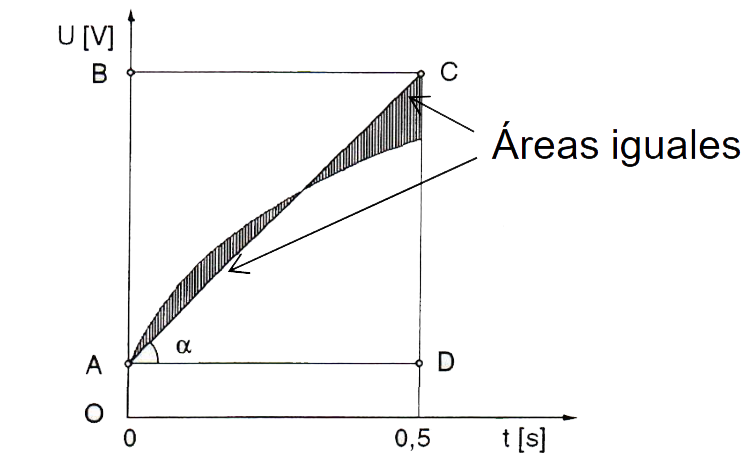
\includegraphics[width=1\linewidth]{res/tema7/tanAlpha}
				\end{minipage}
			\end{figure}
			
			En el caso de un cortocircuito en la red, el inducido provoca un campo opuesto al campo principal, lo que provoca que la excitatriz tiene que suministrar una potencia más alta que en servicio nominal. Este exceso de tensión puede estar entre un 40 y un 80\% de la tensión nominal.
					
		\subsection{Clasificación de los sistemas de excitación.}
			\begin{itemize}
				\item Excitación estática o directa:
					\begin{itemize}
						\item Sistema autoexcitado.
						\item Excitación independiente.
					\end{itemize}
				\item Excitación rotativa o indirecta:
					\begin{itemize}
						\item Excitatriz de c.a. con diodos giratorios.
						\item Excitatriz de c.c.
						\item Excitación independiente o autoexcitada.
						\item Chopper o rectificador de alterna con tiristores.
					\end{itemize}
			\end{itemize}
		
			\newpage
			\subsubsection{Excitación estática o directa, autoexcitada con anillos y escobillas.}

						Es un sistema autoexcitado de excitación independiente. Muy habitual en generadores de pequeña potencia. 
						

						Se alimenta el inductor a través de anillos rozantes y escobillas. Es un sistema de respuesta rápida y es autónomo menos en el arranque. 
						

						Tiene la desventaja de tener una respuesta pobre ante cortocircuitos cercanos.

						\begin{figure}[H]
							\centering
							\begin{circuitikz}
								\tikzstyle{every node}=[font=\normalsize]
								\draw  (13,14.25) circle (0.75cm);
								\draw  (13,13.5) circle (0.75cm);
								\draw  (14.5,11.75) circle (0.5cm);
								\draw  (15,11.75) circle (0.5cm);
								\draw (17.5,10.5) to[D] (16.5,10.5);
								\draw  (16.25,11) rectangle (17.75,10);
								\draw  (13,9.25) circle (1.5cm);
								\draw  (13,9.25) circle (1cm) node {\normalsize Rotor} ;
								\node [font=\normalsize] at (13,7.5) {Estátor};
								\draw [](13,10.75) to[short] (13,12.75);
								\draw[] (14,11.75) to[short] (13,11.75);
								\node at (13,11.75) [circ] {};
								\node [font=\normalsize] at (14.75,12.9) {Transformador};
								\node [font=\normalsize] at (14.75,12.5) {de excitación};
								\node [font=\normalsize, rotate around={90:(0,0)}] at (11.55,14) {Transformador};
								\node [font=\normalsize, rotate around={90:(0,0)}] at (12,14) {de potencia};
								\draw [](13,15) to[short] (13,16);
								\draw [](12.75,15.75) to[short] (13.25,15.75);
								\node [font=\normalsize, rotate around={-360:(0,0)}] at (14.75,15.75) {Red de transporte};
								\node [font=\normalsize, rotate around={-360:(0,0)}] at (15.25,10.6) {Puente de};
								\draw [](15.5,11.75) to[short] (17,11.75);
								\draw [](17,11.75) to[short] (17,11);
								\draw [](17,10) to[short] (17,9.25);
								\draw[] (17,9.25) to[short] (14,9.25);
								\node [font=\normalsize, rotate around={-360:(0,0)}] at (15.25,10.25) {tiristores};
								\node [font=\normalsize, rotate around={-360:(0,0)}] at (16.25,12) {c.a.};
								\node [font=\normalsize, rotate around={-360:(0,0)}] at (15.75,9.5) {c.c.};
								\draw [, rotate around={-360:(19.625, 10.5)}] (19,11) rectangle  node {\normalsize AVR} (20.25,10);
								\draw (19,10.5) to[short] (17.75,10.5);
							\end{circuitikz}
							
							\label{fig:my_label}
						\end{figure}
				
		\subsubsection{Excitación estática o directa, con excitación independiente a través de servicios auxiliares.}

					Se alimenta de la red de servicios auxiliares o similar. 
					

					Muy habitual en generadores de pequeña potencia. Utiliza escobillas y anillos rozantes. Respuesta rápida. 
					

					Tiene la desventaja de tener una respuesta pobre ante cortocircuitos cercanos en la red.

					\begin{figure}[H]
						\centering
							\begin{circuitikz}
								\tikzstyle{every node}=[font=\LARGE]
								\draw  (13,14.25) circle (0.75cm);
								\draw  (13,13.5) circle (0.75cm);
								\draw  (17,13.25) circle (0.5cm);
								\draw  (17,12.75) circle (0.5cm);
								\draw (17.5,10.5) to[D] (16.5,10.5);
								\draw  (16.25,11) rectangle (17.75,10);
								\draw  (13,9.25) circle (1.5cm);
								\draw  (13,9.25) circle (1cm) node {\normalsize Rotor} ;
								\node [font=\normalsize] at (13,7.5) {Estátor};
								\draw [](13,10.75) to[short] (13,12.75);
								\node [font=\normalsize, rotate around={90:(0,0)}] at (15.9,13) {Servicios};
								\node [font=\normalsize, rotate around={90:(0,0)}] at (16.25,13) {auxiliares};
								\node [font=\normalsize, rotate around={90:(0,0)}] at (11.55,14) {Transformador};
								\node [font=\normalsize, rotate around={90:(0,0)}] at (12,14) {de potencia};
								\draw [](13,15) to[short] (13,16);
								\draw [](12.75,15.75) to[short] (13.25,15.75);
								\node [font=\normalsize, rotate around={-360:(0,0)}] at (14.75,15.75) {Red de transporte};
								\node [font=\normalsize, rotate around={-360:(0,0)}] at (15.25,10.6) {Puente de};
								\draw [](17,12.25) to[short] (17,11.75);
								\draw [](17,11.75) to[short] (17,11);
								\draw [](17,10) to[short] (17,9.25);
								\draw[] (17,9.25) to[short] (14,9.25);
								\node [font=\normalsize, rotate around={-360:(0,0)}] at (15.25,10.25) {tiristores};
								\node [font=\normalsize, rotate around={90:(0,0)}] at (16.75,11.75) {c.a.};
								\node [font=\normalsize, rotate around={-360:(0,0)}] at (15.75,9.5) {c.c.};
								\draw [, rotate around={-360:(19.625, 10.5)}] (19,11) rectangle  node {\normalsize AVR} (20.25,10);
								\draw[] (19,10.5) to[short] (17.75,10.5);
								\draw [](17,13.75) to[short] (17,14.5);
							\end{circuitikz}
						
						\label{fig:my_label}
					\end{figure}

		\newpage
			
		\subsubsection{Excitación rotativa o indirecta, con excitatriz de c.c. sin excitatriz piloto.}
					Una máquina de c.c. alimenta el inductor a través de anillos rozantes y escobillas. Unida al eje del generador.
					

					Para generadores hidráulicos de hasta $50\,MV\!A$. 
					

					Alimentación independiente mediante red auxiliar.
					\vspace{0.5cm}
					\begin{figure}[H]
						\centering
							\begin{circuitikz}
								\tikzstyle{every node}=[font=\normalsize]
								\draw  (13,14.25) circle (0.75cm);
								\draw  (13,13.5) circle (0.75cm);
								\draw  (18.5,14) circle (0.5cm);
								\draw  (18.5,13.5) circle (0.5cm);
								\draw (19,11.25) to[D] (18,11.25);
								\draw  (17.75,11.75) rectangle (19.25,10.75);
								\draw  (13,9.25) circle (1.5cm);
								\draw  (13,9.25) circle (1cm) node {\normalsize Generador} ;
								\draw [](13,10.75) to[short] (13,12.75);
								\node [font=\normalsize, rotate around={90:(0,0)}] at (17.4,13.75) {Servicios};
								\node [font=\normalsize, rotate around={90:(0,0)}] at (17.75,13.75) {auxiliares};
								\node [font=\normalsize, rotate around={90:(0,0)}] at (11.55,14) {Transformador};
								\node [font=\normalsize, rotate around={90:(0,0)}] at (12,14) {de potencia};
								\draw [](13,15) to[short] (13,16);
								\draw [](12.75,15.75) to[short] (13.25,15.75);
								\node [font=\normalsize, rotate around={-360:(0,0)}] at (14.75,15.75) {Red de transporte};
								\node [font=\normalsize, rotate around={-360:(0,0)}] at (16.75,11.3) {Puente de};
								\draw [](18.5,13) to[short] (18.5,12.5);
								\draw [](18.5,12.5) to[short] (18.5,11.75);
								\draw [](18.5,10.75) to[short] (18.5,10);
								\node [font=\normalsize, rotate around={-360:(0,0)}] at (16.75,11) {tiristores};
								\node [font=\normalsize, rotate around={90:(0,0)}] at (18.25,12.5) {c.a.};
								\draw [, rotate around={-360:(21.125, 11.25)}] (20.5,11.75) rectangle  node {\normalsize AVR} (21.75,10.75);
								\draw[] (20.5,11.25) to[short] (19.25,11.25);
								\draw [](18.5,14.5) to[short] (18.5,15.25);
								
								\draw  (16.5,9.25) circle (0.5cm);
								\draw  (16.5,9.25) circle (0.75cm) node {\normalsize Exc.} ;
								\draw [dashed] (14,9.25) -- (16,9.25);
								\draw [short] (13.75,9.875) -- (14.5,10.5);
								\draw [short] (13.75,8.625) -- (14.5,8);
								\draw [short] (14.5,10.5) -- (16.5,10.5);
								\draw [short] (16.5,10.5) -- (16.5,10);
								\draw [short] (16.5,8.5) -- (16.5,8);
								\draw [short] (16.5,8) -- (14.5,8);
								\node at (16.5,10) [circ] {};
								\node at (16.5,8.5) [circ] {};
								\draw [ fill={rgb,255:red,0; green,0; blue,0} , rotate around={-360:(17.625, 9.25)}] (17.5,10) rectangle (17.75,8.5);
								\draw [](18.5,10) to[short] (18.5,9.25);
								\draw[] (18.5,9.25) to[short] (17.75,9.25);
								\node [font=\normalsize, rotate around={90:(0,0)}] at (18.25,10) {c.c.};
								\node [font=\normalsize, rotate around={-360:(0,0)}] at (15.25,8.25) {c.c.};
							\end{circuitikz}
						
						\label{fig:my_label}
					\end{figure}
					\vspace{1cm}
		\subsubsection{Excitación rotativa o indirecta, con excitatriz principal y piloto de c.c.}
			Muy habitual en generadores de baja velocidad y media potencia, hasta $50\,MV\!A$.
			
			
			Excitatriz piloto y principal de c.c.
			
			
			Sistema autónomo. No depende de la red, sólo se necesita hacer girar el eje común a las 3 máquinas. Se alimenta a través de anillos y escobillas.
			
			
			Respuesta más lenta y mayor coste de mantenimiento por las escobillas.
			\vspace{0.5cm}
			\begin{figure}[H]
				\centering
				\begin{circuitikz}
					\tikzstyle{every node}=[font=\normalsize]
					\draw  (10,12.75) circle (1.5cm);
					\draw  (10,12.75) circle (1cm);
					\draw (10,13.5) to[L ] (10,12);
					\draw [dashed] (10,12.75) -- (18.5,12.75);
					\draw [ fill={rgb,255:red,0; green,0; blue,0} , rotate around={-360:(12.625, 12.75)}] (12.5,13.25) rectangle (12.75,12.25);
					\draw [ fill={rgb,255:red,0; green,0; blue,0} , rotate around={-360:(13.125, 12.75)}] (13,13.25) rectangle (13.25,12.25);
					\draw  (15,12.75) circle (0.5cm);
					\node at (15,13.25) [circ] {};
					\node at (15,12.25) [circ] {};
					\draw [](10,12) to[short] (11.75,12);
					\draw [](11.75,12) to[short] (11.75,12.25);
					\draw [](11.75,12.25) to[short] (11.75,12.5);
					\draw [](11.75,12.5) to[short] (13,12.5);
					\draw [](10,13.5) to[short] (11.75,13.5);
					\draw [](11.75,13.5) to[short] (11.75,13);
					\draw [](11.75,13) to[short] (12.5,13);
					\draw [](12.625,13.25) to[short] (12.625,13.75);
					\draw [](12.625,13.75) to[short] (15,13.75);
					\draw [](15,13.75) to[short] (15,13.25);
					\draw [](15,12.25) to[short] (15,11.75);
					\draw[] (15,11.75) to[short] (13.125,11.75);
					\draw [](13.125,11.75) to[short] (13.125,12.25);
					\draw (16,13.5) to[L ] (16,12);
					\draw  (18.5,12.75) circle (0.5cm);
					\draw [](18.5,13.25) to[short] (18.5,13.75);
					\draw [](18.5,12.25) to[short] (18.5,11.75);
					\draw (16,13.75) to[R] (17.5,13.75);
					\draw [->, >=Stealth] (16.75,14.5) -- (16.75,14);
					\draw [short] (16.75,14.5) -- (18.5,14.5);
					\draw [short] (18.5,14.5) -- (18.5,13.75);
					\draw [short] (16,13.75) -- (16,13.5);
					\draw [short] (18.5,11.75) -- (16,11.75);
					\draw [short] (16,11.75) -- (16,12);
					\draw (19.5,13.5) to[L ] (19.5,12);
					\draw [](19.5,13.5) to[short] (19.5,14.5);
					\draw[] (19.5,14.5) to[short] (18.5,14.5);
					\draw [](18.5,11.75) to[short] (19.5,11.75);
					\draw [](19.5,11.75) to[short] (19.5,12);
					\node at (18.5,14.5) [circ] {};
					\node at (18.5,11.75) [circ] {};
					\node [font=\normalsize, rotate around={-360:(0,0)}] at (18.25,13.5) {+};
					\node [font=\normalsize, rotate around={-360:(0,0)}] at (14.75,13.5) {+};
					\node [font=\normalsize, rotate around={-360:(0,0)}] at (15.5,11.4) {Excitatriz};
					\node [font=\normalsize, rotate around={-360:(0,0)}] at (15.5,11.1) {principal};
					\node [font=\normalsize, rotate around={-360:(0,0)}] at (19,11.4) {Excitatriz};
					\node [font=\normalsize, rotate around={-360:(0,0)}] at (19,11.1) {piloto};
					\draw (7,12.75) to[tmultiwire= \normalsize Red] (8.5,12.75);
				\end{circuitikz}
				
				\label{fig:my_label}
			\end{figure}
		\newpage
		\subsubsection{Excitación rotativa o indirecta, con excitatriz de c.a. y piloto de imanes permanentes}
			Potencias de hasta $50\,MV\!A$.
			
			
			Se necesitan anillos y escobillas en el alternador principal, pero no en las excitatrices.
			
			
			Sistema autónomo de la red: sólo es necesario girar el eje de la turbina.
			
			
			Tiempo de respuesta lento, coste de mantenimiento alto por las escobillas, y no es aconsejable subir de 1500 $rpm$ por la resistencia mecánica en las escobillas.
			\vspace{0.5cm}
			\begin{figure}[H]
				\centering
				\begin{circuitikz}
					\tikzstyle{every node}=[font=\normalsize]
					\draw  (10,12.75) circle (1.5cm);
					\draw  (10,12.75) circle (1cm);
					\draw (10,13.5) to[L ] (10,12);
					\draw [dashed] (10,12.75) -- (18,12.75);
					\draw [ fill={rgb,255:red,0; green,0; blue,0} , rotate around={-360:(12.625, 12.75)}] (12.5,13.25) rectangle (12.75,12.25);
					\draw [ fill={rgb,255:red,0; green,0; blue,0} , rotate around={-360:(13.125, 12.75)}] (13,13.25) rectangle (13.25,12.25);
					\draw [](10,12) to[short] (11.75,12);
					\draw [](11.75,12) to[short] (11.75,12.25);
					\draw [](11.75,12.25) to[short] (11.75,12.5);
					\draw [](11.75,12.5) to[short] (13,12.5);
					\draw [](10,13.5) to[short] (11.75,13.5);
					\draw [](11.75,13.5) to[short] (11.75,13);
					\draw [](11.75,13) to[short] (12.5,13);
					\draw [](13.125,13.25) to[short] (13.125,14.5);
					\draw [](7,12.75) to[tmultiwire= \normalsize Red] (8.5,12.75);
					\draw (15,14.75) to[D] (14,14.75);
					\draw [, rotate around={-360:(14.5, 14.75)}] (13.75,15.25) rectangle (15.25,14.25);
					\draw [short] (13.125,14.5) -- (13.75,14.5);
					\draw [short] (13.75,15) -- (12.625,15);
					\draw [short] (12.625,15) -- (12.625,13.25);
					\draw [short] (15.25,14.75) -- (16.25,14.75);
					\draw  (16.25,12.75) circle (1cm);
					\draw  (16.25,12.75) circle (1.25cm);
					\draw [](16.25,13.74) to[tmultiwire] (16.25,14.75);
					\draw [](17.25,13.5) to[short] (18,13.5);
					\draw [](17.25,12) to[short] (18,12);
					\draw (18.5,12.25) to[D] (18.5,13.25);
					\draw [, rotate around={-360:(18.5, 12.75)}] (18,13.75) rectangle (19,11.75);
					\draw [dashed] (19,12.75) -- (20.5,12.75);
					\draw  (21,12.75) circle (0.75cm) node {\normalsize G} ;
					\draw  (21,12.75) circle (0.5cm);
					\draw[] (21,14.25) to[tmultiwire] (18.5,14.25);
					\draw [](21,14.25) to[short] (21,13.5);
					\draw [](18.5,14.25) to[short] (18.5,13.75);
					\node [font=\normalsize, rotate around={-360:(0,0)}] at (16.75,11.25) {Excitatriz principal};
					\node [font=\normalsize, rotate around={-360:(0,0)}] at (16.75,10.85) {de corriente alterna};
					\node [font=\normalsize, rotate around={-360:(0,0)}] at (21,11.25) {Excitatriz piloto};
					\node [font=\normalsize, rotate around={-360:(0,0)}] at (21,10.8) {de imanes permanentes};
					\node [font=\normalsize, rotate around={-360:(0,0)}] at (10,11) {Alternador};
				\end{circuitikz}
				
				\label{fig:my_label}
			\end{figure}
		
		
		\subsubsection{Excitación rotativa o indirecta, con generador auxiliar de c.a. de imanes permanentes.}

					Potencias de hasta $50\,MV\!A$.
					

					Se alimenta el inductor con una excitatriz de imanes permanentes de c.a acoplada en el mismo eje. Al ser de imanes permanentes el flujo en la excitatriz es constante. El inductor del generador síncrono se alimenta a través de escobillas y anillos rozantes.
					

					Sistema más rápido de actuación. Autónomo, pues sólo se necesita mover el eje con la turbina.
					\vspace{0.5cm}
					\begin{figure}[H]
						\centering
						\begin{circuitikz}
							\tikzstyle{every node}=[font=\normalsize]
							\draw  (13,14.25) circle (0.75cm);
							\draw  (13,13.5) circle (0.75cm);
							\draw (16.75,11.25) to[D] (15.75,11.25);
							\draw  (15.5,11.75) rectangle (17,10.75);
							\draw  (13,9.25) circle (1.5cm);
							\draw  (13,9.25) circle (1cm) node {\normalsize Generador} ;
							\draw [](13,10.75) to[short] (13,12.75);
							\node [font=\normalsize, rotate around={90:(0,0)}] at (11.55,14) {Transformador};
							\node [font=\normalsize, rotate around={90:(0,0)}] at (12,14) {de potencia};
							\draw [](13,15) to[short] (13,16);
							\draw [](12.75,15.75) to[short] (13.25,15.75);
							\node [font=\normalsize, rotate around={-360:(0,0)}] at (14.75,15.75) {Red de transporte};
							\node [font=\normalsize, rotate around={-360:(0,0)}] at (16.25,10.5) {Puente de};
							\node [font=\normalsize, rotate around={-360:(0,0)}] at (16.25,10.175) {tiristores};
							
							\draw  (19.5,9.25) circle (0.5cm);
							\draw  (19.5,9.25) circle (0.75cm) node {\normalsize G} ;
							\draw [dashed] (14,9.25) -- (19,9.25);
							\draw [short] (13.75,9.875) -- (15,11.25);
							\draw [short] (15,11.25) -- (15.5,11.25);
							\draw [short] (17,11.25) -- (17.5,11.25);
							\draw [short] (17.5,11.25) -- (18.95,9.75);
							\draw [, rotate around={-360:(16.25, 12.75)}] (15.5,13.25) rectangle  node {\normalsize AVR} (17,12.25);
							\draw [](16.25,12.25) to[short] (16.25,11.75);
							\node [font=\normalsize, rotate around={-360:(0,0)}] at (19.5,10.75) {Imanes};
							\node [font=\normalsize, rotate around={-360:(0,0)}] at (19.5,10.5) {Permanentes};
						\end{circuitikz}
						
						\label{fig:my_label}
					\end{figure}

		\newpage
		\subsubsection{Excitación rotativa o indirecta, sin escobillas con diodos giratorios y excitatriz de c.a.}
			Para generadores de alta potencia y respuesta rápida.
			
			
			El inductor del generador, la caja de diodos y el inductor de c.a. de la excitatriz están en el mismo eje. El devanado de excitación de la excitatriz de corriente alterna se alimenta mediante una red independiente o auxiliar.
			
			
			Tiene el inconveniente de dar una respuesta pobre ante cortocircuitos en la red auxiliar.
			
			\vspace{0.25cm}
			\textbf{\textit{Diodos giratorios:}}
			\begin{itemize}
				\item Giran solidarios al eje.
				\item El eje del generado es hueco para poder pasar los cables que vienen del puente rectificador.
				\item La excitatriz principal genera una tensión trifásica con una frecuencia del orden de los $350\,Hz$, para disminuir el rizado. La excitatriz piloto de c.a. genera una tensión trifásica con una frecuencia del orden de los $250\,Hz$.
				\item El puente rectificador de diodos giratorios puede contener cerca de 60 diodos rectificadores, montados en serie y paralelo. Cada diodo lleva asociado un fusible de protección contra cortocircuitos, y puede haber 30 grupos R-C de protección contra sobretensiones.
			\end{itemize}
			
			\begin{figure}[H]
				\centering
					\begin{circuitikz}
						\tikzstyle{every node}=[font=\normalsize]
						\draw  (13,14.25) circle (0.75cm);
						\draw  (13,13.5) circle (0.75cm);
						\draw  (19.75,14) circle (0.5cm);
						\draw  (19.75,13.5) circle (0.5cm);
						\draw (20.25,11.25) to[D] (19.25,11.25);
						\draw  (19,11.75) rectangle (20.5,10.75);
						\draw  (13,9.25) circle (1.5cm);
						\draw  (13,9.25) circle (1cm) node {\normalsize Generador} ;
						\draw [](13,10.75) to[short] (13,12.75);
						\node [font=\normalsize, rotate around={90:(0,0)}] at (18.7,13.75) {Servicios};
						\node [font=\normalsize, rotate around={90:(0,0)}] at (19,13.75) {auxiliares};
						\node [font=\normalsize, rotate around={90:(0,0)}] at (11.65,14) {Transformador};
						\node [font=\normalsize, rotate around={90:(0,0)}] at (12,14) {de potencia};
						\draw [](13,15) to[short] (13,16);
						\draw [](12.75,15.75) to[short] (13.25,15.75);
						\node [font=\normalsize, rotate around={-360:(0,0)}] at (14.75,15.75) {Red de transporte};
						\node [font=\normalsize, rotate around={-360:(0,0)}] at (18,11.3) {Puente de};
						\draw [](19.75,13) to[short] (19.75,12.5);
						\draw [](19.75,12.5) to[short] (19.75,11.75);
						\draw [](19.75,10.75) to[short] (19.75,10);
						\node [font=\normalsize, rotate around={-360:(0,0)}] at (18,11) {tiristores};
						\node [font=\normalsize, rotate around={90:(0,0)}] at (19.5,12.5) {c.a.};
						\draw [, rotate around={-360:(22.375, 11.25)}] (21.75,11.75) rectangle  node {\normalsize AVR} (23,10.75);
						\draw[] (21.75,11.25) to[short] (20.5,11.25);
						\draw [](19.75,14.5) to[short] (19.75,15.25);
						
						\draw  (18.25,9.25) circle (0.5cm);
						\draw  (18.25,9.25) circle (0.75cm) node {\normalsize Exc.} ;
						\draw [short] (14,9.25) -- (15.25,9.25);
						\draw [](19.75,10) to[short] (19.75,9.25);
						\draw[] (19.75,9.25) to[short] (19,9.25);
						\node [font=\normalsize, rotate around={90:(0,0)}] at (19.5,10) {c.c.};
						\draw  (15.25,9.75) rectangle (16.75,8.75);
						\draw (16.5,9.25) to[D] (15.5,9.25);
						\draw [](16.75,9.25) to[short] (17.75,9.25);
						\node [font=\normalsize, rotate around={-360:(0,0)}] at (16,10.5) {Caja de};
						\node [font=\normalsize, rotate around={-360:(0,0)}] at (16,10.15) {diodos giratorios};
						\node [font=\normalsize, rotate around={-360:(0,0)}] at (17.2,9.5) {c.a.};
						\node [font=\normalsize, rotate around={-360:(0,0)}] at (14.85,9.5) {c.c.};
					\end{circuitikz}
				
				\label{fig:my_label}
			\end{figure}
		
		\subsubsection{Excitación rotativa o indirecta, con diodos giratorios, excitatriz de c.a. y excitatriz piloto de imanes permanentes.}
			Sistema de excitación para generadores de alta potencia de respuesta un poco más lenta. 
			
			
			El inductor del generador síncrono, la caja de diodos giratorios y el inductor de c.a de la excitatriz principal están en el mismo eje. El devanado de excitación de la excitatriz de corriente alterna se alimenta mediante un generador de imanes permanentes (flujo constante). El inductor del generador no tiene escobillas ni anillos rozantes. Se alimenta mediante los diodos rectificadores giratorios, a través del eje del generador que está hueco.
			
			
			Sistema autónomo de la red. No le influyen los cortocircuitos en la red.
			
			\begin{figure}[H]
				\centering
				\begin{circuitikz}
					\tikzstyle{every node}=[font=\normalsize]
					\draw (22.75,10.5) to[D] (21.75,10.5);
					\draw  (21.5,11) rectangle (23,10);
					\draw  (13,9.75) circle (1.5cm);
					\draw  (13,9.75) circle (1cm) node {\normalsize Generador} ;
					\node [font=\normalsize, rotate around={-360:(0,0)}] at (24,11.25) {Puente de tiristores};
					
					\draw  (18.25,9.75) circle (0.5cm);
					\draw  (18.25,9.75) circle (0.75cm) node {\normalsize Exc.} ;
					\draw [short] (14,9.75) -- (15.25,9.75);
					\draw[] (21.5,10.5) to[short] (21,10.5);
					\node [font=\normalsize, rotate around={-360:(0,0)}] at (20.75,10.75) {c.c.};
					\draw  (15.25,10.25) rectangle (16.75,9.25);
					\draw (16.5,9.75) to[D] (15.5,9.75);
					\draw [](16.75,9.75) to[short] (17.75,9.75);
					\node [font=\normalsize, rotate around={-360:(0,0)}] at (16,8.75) {Caja de};
					\node [font=\normalsize, rotate around={-360:(0,0)}] at (16,8.375) {diodos giratorios};
					\node [font=\normalsize, rotate around={-360:(0,0)}] at (17.2,9.5) {c.a.};
					\node [font=\normalsize, rotate around={-360:(0,0)}] at (14.85,9.5) {c.c.};
					\draw  (10.25,9.75) circle (0.5cm) node {\normalsize M} ;
					\draw [dashed] (10.75,9.75) -- (12,9.75);
					\draw  (21.5,12.25) rectangle  node {\normalsize AVR} (23,11.5);
					\draw [short] (22.25,11.5) -- (22.25,11);
					\draw (19,9.75) to[R] (21,9.75);
					\draw [->, >=Stealth] (20,10.5) -- (20,10);
					\draw [short] (20,10.5) -- (21,10.5);
					\draw [](13,11.25) to[tmultiwire= \normalsize Red] (13,12.25);
					\draw  (24.5,9.75) circle (0.5cm) node {\normalsize G} ;
					\draw [dashed] (24,9.75) -- (21.25,9.75);
					\draw [](23,10.5) to[tmultiwire] (24.5,10.5);
					\draw [](24.5,10.5) to[short] (24.5,10.25);
					\node [font=\normalsize] at (10.25,11) {Motor};
					\node [font=\normalsize] at (10.25,10.625) {primario};
					\node [font=\normalsize] at (24.5,9) {Excitatriz piloto};
					\node [font=\normalsize] at (24.5,8.625) {de imanes permanentes};
					\node [font=\normalsize] at (18.25,11.5) {Excitatriz principal};
					\node [font=\normalsize] at (18.25,11.125) {de corriente};
					\node [font=\normalsize] at (18.25,10.75) {alterna};
				\end{circuitikz}
				
				\label{fig:my_label}
			\end{figure}
		
		\subsubsection{Sistema de autoexcitación con excitatriz de c.a. y diodos giratorios.}
			Muy habitual en generadores de gran potencia.
		
		
			El sistema de excitación se alimenta de la tensión en bornes del generador a través del transformador trifásico de excitación, que alimenta el puente controlado de tiristores o IGBTs.
		
			
			Sistema autónomo, salvo en los arranques. Respuesta rápida.
			
			
			Respuesta pobre cuando hay cortocircuitos cercanos en la red.
			
			
			\vspace{0.25cm}
			\textbf{\textit{Proceso de arranque:}}
			
			
			Dado que el regulador de tensión (AVR) no puede funcionar con la pequeña tensión generada por el magnetismo remanente del generador síncrono, es necesario disponer de una fuente de alimentación independiente que alimente el inductor del generador solamente durante el proceso de arranque.
			
			
			Puede hacerse mediante baterías o una red auxiliar independiente, con un transformador de arranque.
					
			\begin{figure}[H]
				\centering
				\begin{circuitikz}
					\tikzstyle{every node}=[font=\normalsize]
					\draw  (13,14.25) circle (0.75cm);
					\draw  (13,13.5) circle (0.75cm);
					\draw  (15.75,12) circle (0.5cm);
					\draw  (16.25,12) circle (0.5cm);
					\draw (20.25,10.75) to[D] (19.25,10.75);
					\draw  (19,11.25) rectangle (20.5,10.25);
					\draw  (13,9.25) circle (1.5cm);
					\draw  (13,9.25) circle (1cm) node {\normalsize Generador} ;
					\draw [](13,10.75) to[short] (13,12.75);
					\node [font=\normalsize, rotate around={-360:(0,0)}] at (16,13.1) {Transformador};
					\node [font=\normalsize, rotate around={-360:(0,0)}] at (16,12.75) {de excitación};
					\node [font=\normalsize, rotate around={90:(0,0)}] at (11.65,14) {Transformador};
					\node [font=\normalsize, rotate around={90:(0,0)}] at (12,14) {de potencia};
					\draw [](13,15) to[short] (13,16);
					\draw [](12.75,15.75) to[short] (13.25,15.75);
					\node [font=\normalsize, rotate around={-360:(0,0)}] at (14.75,15.75) {Red de transporte};
					\node [font=\normalsize, rotate around={-360:(0,0)}] at (18,11) {Puente de};
					\draw [](19.75,12) to[short] (19.75,11.25);
					\draw [](19.75,10.25) to[short] (19.75,10);
					\node [font=\normalsize, rotate around={-360:(0,0)}] at (18,10.6) {tiristores};
					\node [font=\normalsize, rotate around={-360:(0,0)}] at (18.25,12.25) {c.a.};
					\draw [, rotate around={-360:(22.375, 10.75)}] (21.75,11.25) rectangle  node {\normalsize AVR} (23,10.25);
					\draw[] (21.75,10.75) to[short] (20.5,10.75);
					
					\draw  (18.25,9.25) circle (0.5cm);
					\draw  (18.25,9.25) circle (0.75cm) node {\normalsize Exc.} ;
					\draw [short] (14,9.25) -- (15.25,9.25);
					\draw [](19.75,10) to[short] (19.75,9.25);
					\draw[] (19.75,9.25) to[short] (19,9.25);
					\node [font=\normalsize, rotate around={90:(0,0)}] at (19.5,9.75) {c.c.};
					\draw  (15.25,9.75) rectangle (16.75,8.75);
					\draw (16.5,9.25) to[D] (15.5,9.25);
					\draw [](16.75,9.25) to[short] (17.75,9.25);
					\node [font=\normalsize, rotate around={-360:(0,0)}] at (16,10.5) {Caja de};
					\node [font=\normalsize, rotate around={-360:(0,0)}] at (16,10.15) {diodos giratorios};
					\node [font=\normalsize, rotate around={-360:(0,0)}] at (17.2,9.5) {c.a.};
					\node [font=\normalsize, rotate around={-360:(0,0)}] at (14.85,9.5) {c.c.};
					\draw [](16.75,12) to[short] (19.75,12);
					\draw[] (15.25,12) to[short] (13,12);
					\node at (13,12) [circ] {};
				\end{circuitikz}
				
				\label{fig:my_label}
			\end{figure}
		
	\subsection{Cortocircuitos en la red.}	
		Constituye un problema importante, pues en este caso la tensión de alimentación de la excitación desaparece total o parcialmente, en función de la impedancia que pueda haber entre el generador y el punto de defecto.
		
		
		Si el alternador está conectado directamente a un juego de barras, del que se alimentan una serie de cargas y se produce un cortocircuito en una de las líneas, ésta debe ser automáticamente desconectada de forma selectiva y en un tiempo muy breve a fin de no dejar sin suministro el resto de las cargas. En el caso de un alternador autoexcitado, la $I_{cc}$ decrece rápidamente debido a la reducción de la $I_{ex}$ provocada por la reducción de la tensión.
		
	\section{Regulador de tensión (AVR).}
		Tiene como misión:
		\begin{itemize}
			\item Mantener la tensión en bornes del generador dentro de los márgenes permitidos, independientemente del nivel de carga. Normalmente $\pm5\%$ de la tensión nominal.
			\item Regular la potencia reactiva, subexcitando y sobreexcitando al alternador. El generador debe ser capaz de dar un $\pm15\%$ de la potencia activa neta en reactiva.
			\item Mantener el sincronismo del alternador con la red en el caso de un cortocircuito.
			\item Funciones de protección para no sobrepasar los límites de funcionamiento de la máquina.
		\end{itemize}
		
		\subsection{Funciones de regulación y protección del AVR.}
			
	
	\begin{figure}[H]
		\centering
		\begin{circuitikz}
			\tikzstyle{every node}=[font=\normalsize]
			\draw [short] (7.25,10.25) -- (7.25,8.75);
			\draw [short] (6.25,9.25) -- (7.25,8.75);
			\draw [short] (6.25,9.75) -- (7.25,10.25);
			\node [font=\normalsize] at (3.5,10.75) {};
			\node [font=\normalsize] at (6.75,9.5) {TV};
			\draw [short] (7.25,9.75) -- (9,9.75);
			\draw [short] (7.25,9.25) -- (9,9.25);
			\draw [short] (9.75,10) -- (10,10);
			\draw [short] (10,10) -- (10,9.75);
			\draw [short] (9.75,9) -- (10,9);
			\draw [short] (10,9) -- (10,9.25);
			\draw [short] (10,9.25) -- (11.8,9.25);
			\draw [short] (10,9.75) .. controls (12.5,9.75) and (10.25,9.75) .. (11.8,9.75);
			\draw  (12.5,9.5) circle (0.75cm) node {\normalsize G} ;
			\draw [line width=0.2pt, short] (12.25,9.25) .. controls (12.5,9.5) and (12.5,9) .. (12.75,9.25);
			\draw [short] (13.25,9.5) -- (15.5,9.5);
			\draw [short] (14.75,9.5) -- (14.75,7);
			\draw  (11.5,7.5) rectangle (13.5,6.5);
			\node [font=\normalsize] at (12.5,7.25) {Regulador};
			\node [font=\normalsize] at (12.5,6.75) {AVR};
			\draw (11.75,8.25) to[L ] (13.25,8.25);
			\draw [short] (11.75,8.25) -- (11.75,7.5);
			\draw [short] (13.25,8.25) -- (13.25,7.5);
			\draw [line width=0.2pt, short] (13.5,9.25) -- (13.75,9.75);
			\draw [line width=0.2pt, short] (13.75,9.25) -- (14,9.75);
			\draw [line width=0.2pt, short] (14,9.25) -- (14.25,9.75);
			\draw [line width=0.2pt, short] (14.25,9.25) -- (14.5,9.75);
			\draw [short] (9.75,10) -- (9.75,11.25);
			\draw [short] (9.75,10) -- (9.5,10);
			\draw [short] (9.5,10) -- (9.5,9.75);
			\draw [short] (9.5,9.25) -- (9.5,9);
			\draw [short] (9.5,9) -- (9.75,9);
			\draw [short] (9,9.75) -- (9.5,9.75);
			\draw [short] (9,9.25) -- (9.5,9.25);
			\draw [short] (6.25,9.75) -- (6.25,9.25);
			\draw  (8.75,12.25) rectangle (10.75,11.25);
			\node [font=\normalsize] at (9.75,12) {Regulador};
			\node [font=\normalsize] at (9.75,11.5) {velocidad};
			\draw [->, >=Stealth] (8,10) .. controls (8.25,9.5) and (8.25,9.5) .. (8,9) ;
			\draw [->, >=Stealth] (8.75,10) .. controls (9,9.5) and (9,9.5) .. (8.75,9) ;
			\draw [->, >=Stealth] (11.25,9) .. controls (11,9.5) and (11,9.5) .. (11.25,10) ;
			\node [font=\normalsize] at (8,8.75) {n};
			\node [font=\normalsize] at (10,10.75) {n};
			\node [font=\normalsize] at (11.25,10.25) {$T_{elec}$};
			\node [font=\normalsize] at (8.75,8.75) {$T_{mec}$};
			\draw [->, >=Stealth] (9.75,10) -- (9.75,11.25);
			\draw [->, >=Stealth] (12,11.75) -- (10.75,11.75);
			\draw [->, >=Stealth] (12.5,5.75) -- (12.5,6.5);
			\draw [->, >=Stealth] (11.5,7.75) -- (11.5,8.25);
			\draw [->, >=Stealth] (14.75,7) -- (13.5,7);
			\node [font=\normalsize] at (14.75,8.25) {};
			\node [font=\normalsize] at (12.5,5.5) {$V_{ref}$};
			\node [font=\normalsize] at (11.25,8) {$I_{ex}$};
			\node [font=\normalsize] at (15,8) {V};
			\node [font=\normalsize] at (12.5,11.75) {$P_{ref}$};
			\draw  (8,11.75) circle (0.5cm);
			\draw [short] (8.75,11.75) -- (8.5,11.75);
			\node [font=\normalsize] at (8,11.75) {$M$};
			\draw [short] (7.5,11.75) -- (5.75,11.75);
			\draw [->, >=Stealth] (5.75,11.75) -- (5.75,11.25);
			\draw [short] (5.75,11.25) -- (6.25,11.5);
			\draw [short] (5.75,11.25) -- (6.25,11);
			\draw [short] (6.25,11) -- (6.25,11.5);
			\draw [short] (5.75,11.25) -- (5.25,11.5);
			\draw [short] (5.25,11.5) -- (5.25,11);
			\draw [short] (5.25,11) -- (5.75,11.25);
			\draw [short] (6.75,10) -- (6.75,11.25);
			\draw [short] (6.25,11.25) -- (6.75,11.25);
			\draw [short] (5.25,11.25) -- (4.75,11.25);
			\node [font=\normalsize] at (8,12.5) {$Servomotor$};
			\node [font=\normalsize] at (4,11.5) {$Entrada$};
			\node [font=\normalsize] at (4,11) {$vapor$};
			\draw [ color={rgb,255:red,2; green,141; blue,37} , dashed] (10.5,10.75) rectangle  (16,5);
			\draw [ color={rgb,255:red,234; green,72; blue,72}, dashed] (13,10.75) -- (13,13.5);
			\draw [ color={rgb,255:red,234; green,72; blue,72}, dashed] (13,13.5) -- (3.25,13.5);
			\draw [ color={rgb,255:red,234; green,72; blue,72}, dashed] (3.25,13.5) -- (3.25,7.75);
			\draw [ color={rgb,255:red,234; green,72; blue,72}, dashed] (3.25,7.75) -- (10.5,7.75);
			\node [font=\normalsize, color={rgb,255:red,234; green,72; blue,72}] at (4.25,13) {Control P-f};
			\node [font=\normalsize, color={rgb,255:red,62; green,167; blue,89}] at (14.75,5.5) {Control Q-V};
		\end{circuitikz}
		\label{fig:my_label}
	\end{figure}

